\documentclass[prb]{revtex4}% Physical Review B

\usepackage{graphicx}% Include figure files
\usepackage{dcolumn}% Align table columns on decimal point
\usepackage{bm}% bold math
\usepackage{caption}
\usepackage{listings}
\usepackage{hyperref}
%\hypersetup{colorlinks=true} % will remove boxes around hyperlinks and replace them with colored text


%\nofiles

\begin{document}

%\preprint{APS/123-QED}

\title{Introduction to the use the $UB$ matrix} % Force line breaks with \\

\author{A. T. Savici}


\date{\today}% It is always \today, today,
             %  but any date may be explicitly specified

%\begin{abstract}

%\end{abstract}

%\pacs{Valid PACS appear here}% PACS, the Physics and Astronomy
                             % Classification Scheme.
%\keywords{Suggested keywords}%Use showkeys class option if keyword
                              %display desired
\maketitle

\section{$UB$ matrix formalism}

The purpose of using the $UB$ matrix formalism is to map the
scattering geometry in the laboratory frame to the
reciprocal lattice of the sample. Assuming a right handed coordinate
system for the lab frame, and a similar coordinate system tied to the crystal,
the transformation between the two is a simple rotation, $U$.

The physics is described in reciprocal space by $\textbf{Q} = \left(\begin{array}{c}
                                                            h \\
                                                            k \\
                                                            l
                                                          \end{array}\right)$
and energy transfer $E$. The $B$ matrix (shown in section \ref{Bsection}) is the transformation
from $h, k, l$ to a cartesian coordinate system tied to the sample.
\begin{equation}
    \textbf{Q}_c=2 \pi B \left(\begin{array}{c}
                                                            h \\
                                                            k \\
                                                            l
                                                          \end{array}\right)
\end{equation}

To orient the sample, the scattering instrument uses a goniometer with several rotation axes.
The rotation of the sample can be described by
\begin{equation}
 R = R_1(\Omega_1) \cdot R_2(\Omega_2) \cdot \ldots \cdot R_n(\Omega_n)
\end{equation}
where the sample is attached to the rotation axis of $R_n$.

In the most general case, a rotation with angle $\Omega$ around a direction $\textbf{u} = (u_x, u_y, u_z)$, with $u_x^2 +
u_y^2 + u_z^2 = 1$, is described by
\begin{equation}\label{genrot}
    R(\Omega) = \left(
    \begin{array}{ccc}
      \cos(\Omega) + u_x^2 (1 - \cos(\Omega)) & u_x u_y (1 - \cos(\Omega)) - u_z \sin(\Omega) & u_x u_z (1 - \cos(\Omega)) + u_y \sin(\Omega) \\
      u_y u_x (1 - \cos(\Omega)) + u_z \sin(\Omega) & \cos(\Omega) + u_y^2 (1 - \cos(\Omega)) & u_y u_z (1 - \cos(\Omega)) - u_x \sin(\Omega) \\
      u_z u_x (1 - \cos(\Omega)) - u_y \sin(\Omega) & u_z u_y (1 - \cos(\Omega)) + u_x \sin(\Omega) & \cos(\Omega) + u_z^2 (1 - \cos(\Omega))
    \end{array}
                \right)
\end{equation}

When all angles are 0, the rotation matrices are equal to the identity matrix, so the combined effect is still the unit matrix.
\begin{equation}
R(0) = I =
\left(
  \begin{array}{ccc}
    1 & 0 & 0 \\
    0 & 1 & 0 \\
    0 & 0 & 1 \\
  \end{array}
\right)
\end{equation}

In the general case, when all angles of the goniometer are 0, the axes of the orthogonal crystal reciprocal lattice are not aligned
with the axes of the cartesian laboratory frame. The transformation between these two
 can be described by a rotation matrix $U$. Then, our fundamental relations for
transforming between $\textbf{Q}_l$ (in laboratory frame)  and  $\textbf{Q}$ (reciprocal lattice) are:
\begin{eqnarray}
% \nonumber to remove numbering (before each equation)
  \textbf{Q}_l &=& 2 \pi R \cdot U \cdot B \left(\begin{array}{c}
                                                            h \\
                                                            k \\
                                                            l
                                                          \end{array}\right) \label{QUB}\\
  \textbf{Q}_l &=& \textbf{k}_i - \textbf{k}_f \label{consQ}\\
  E &=& \frac{\hbar^2}{2 m}\left(k_i^2 -k_f^2\right) \label{consE}
\end{eqnarray}

Equation \ref{consQ} is the momentum conservation for the lattice, where $\textbf{k}_i, \textbf{k}_f$ are the
incident and final neutron vawevectors, while equation \ref{consE} is the energy transferred to the lattice.

By looking at equation \ref{QUB}, \ref{consQ}, and \ref{consE}, we identify three modes of interacting with the $UB$ matrix:\\
\hspace*{0.25 in} (a) We know $\textbf{k}_i, \textbf{k}_f, U, B$ and $R$. Then we can calculate $h, k, l, E$.\\
\hspace*{0.25 in} (b) We can calculate U and B if we have several reflections.\\
\hspace*{0.25 in} (c) We can rotate the goniometer so as to measure at a particular combination of $h, k, l$, and $E$ in a specific detector.

\section{Conventions}

\

- $a, b, c$ real lattice lengths (in \AA)

- $\alpha, \beta, \gamma$ real lattice angles

- $a^*, b^*, c^*$ reciprocal lattice lengths (in \AA$^{-1}$). We are going to use crystallographic notations (no 2$\pi$ in the definition of reciprocal lattice vectors)

- for any vector $\textbf{v}$, $v$=$|\textbf{v}|$, $\widehat{v}$=$\textbf{v}$/$v$

- incident beam is along $\widehat{z}$ axis, with $\widehat{x}$ in the horizontal plane, and $\widehat{y}$ pointing up (Figure \ref{instgeom}).

- the scattered beam makes an angle $\theta$ with the $\widehat{z}$ axis, and its projection on the  $(\widehat{x},\widehat{y})$ plane
makes an angle $\phi$ with the $\widehat{x}$ axis (Figure \ref{instgeom}).

From equation \ref{consQ}, $\textbf{Q}_l$ can be written as
\begin{equation}\label{Qlab}
\textbf{Q}_l = \left(\begin{array}{c}
                                                            -k_f\sin(\theta)\cos(\phi) \\
                                                            -k_f\sin(\theta)\sin(\phi) \\
                                                            k_i-k_f\cos(\theta)
                                                          \end{array}\right)
\end{equation}
\begin{figure}[hb]
  % Requires \usepackage{graphicx}
  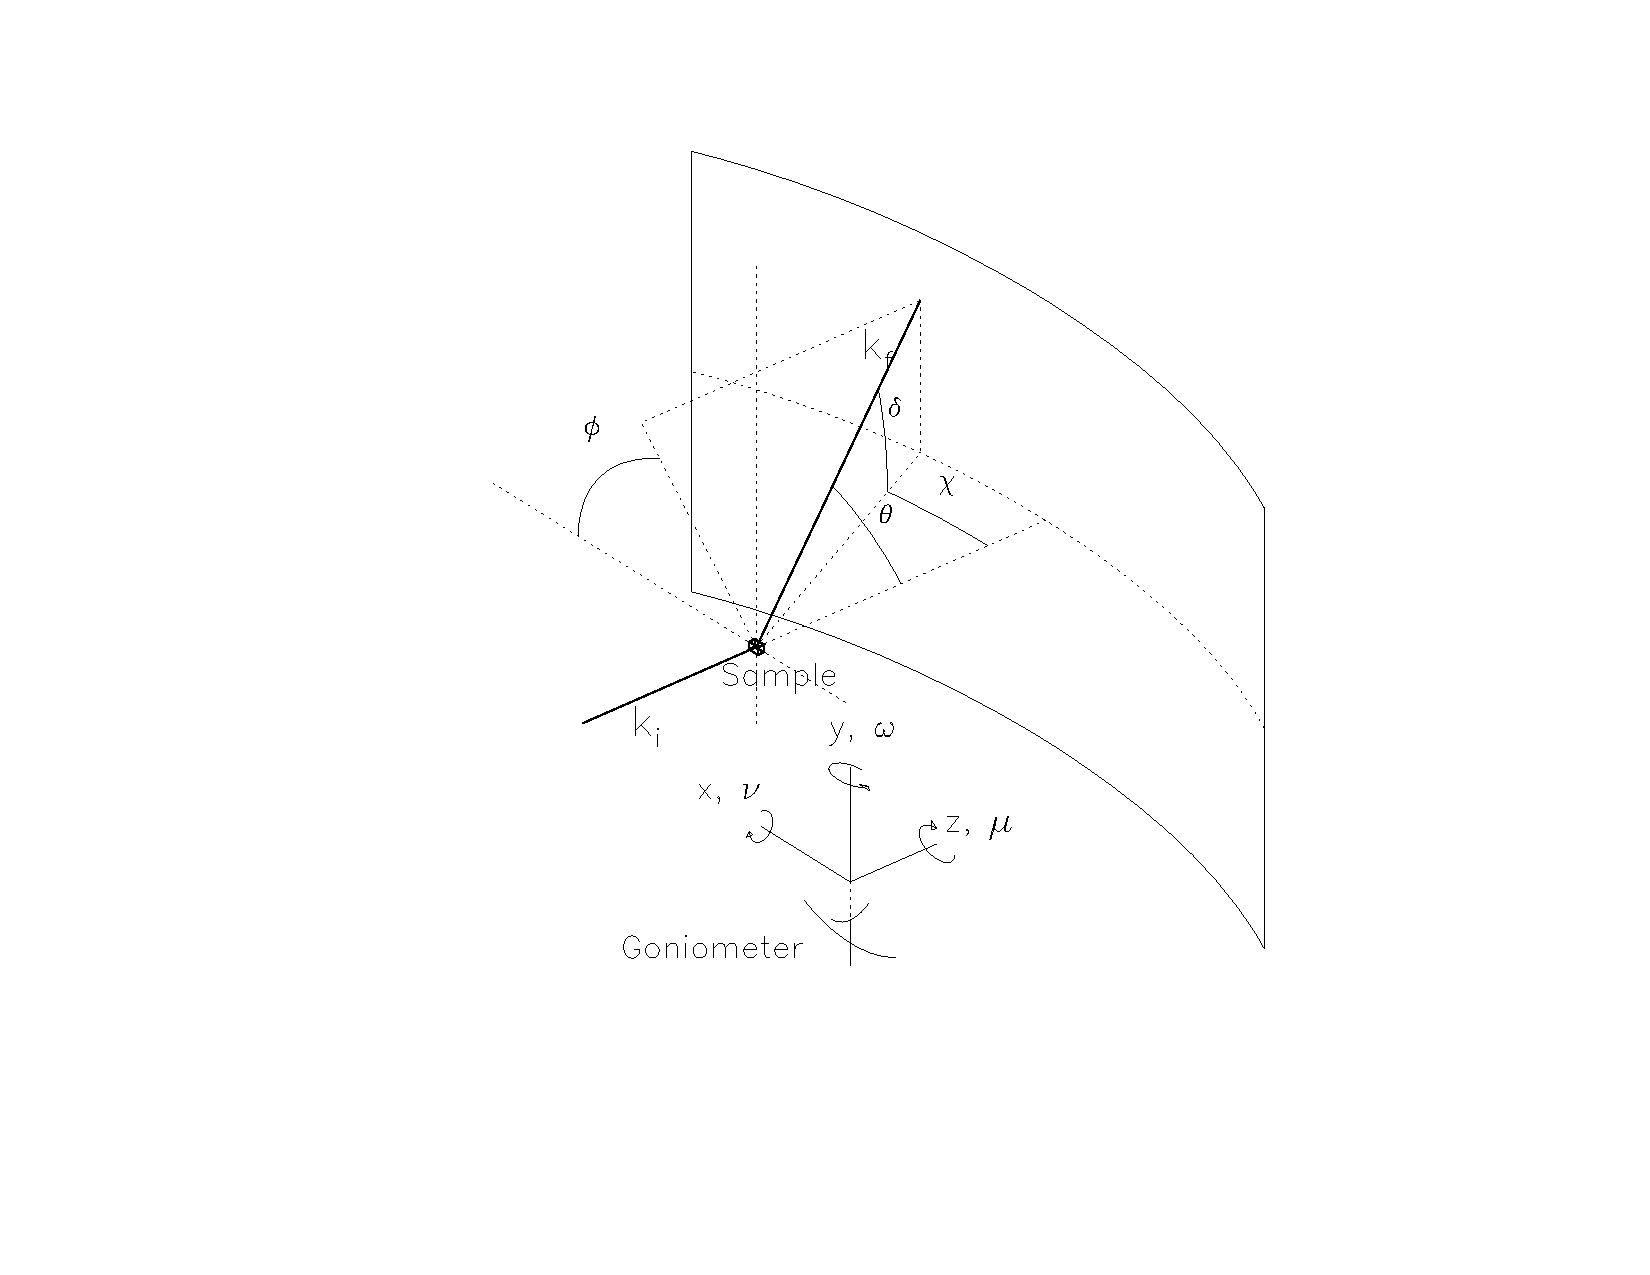
\includegraphics[width=3.5in]{UBmatriximplementationnotes_fig1.pdf}\\
  \caption{Instrument geometry showing conventions for axis and angles.
  Details for goniometer axis are at the bottom}\label{instgeom}
\end{figure}


\section{Reciprocal lattice}

Note: for a more detailed description see \href{http://it.iucr.org/Ba/ch1o1v0001/}{International Tables for Crystallography (2006). Vol. B, ch. 1.1, pp. 2-9 }

This section will contain a description of the calculation of reciprocal lattice parameters. These are useful for
calculating the $B$ matrix, or for extracting real lattice parameters from the $B$ matrix.

Suppose we have an orthonormal set of vectors $\widehat{i}, \widehat{j}, \widehat{k}$, such as
\begin{equation}
    \textbf{a} = a \widehat{i}
\end{equation}
and  $\textbf{b}$ is in the plane of $\widehat{i}$ and $\widehat{j}$, and the angle between $\textbf{a}$ and $\textbf{b}$ is $\gamma$. Then
\begin{equation}
    \textbf{b} = b \cos(\gamma) \widehat{i} + b \sin(\gamma)
    \widehat{j}
\end{equation}
For the $\textbf{c}$ vector, it is slightly more complicated. We write
\begin{equation}
    \textbf{c} = c_i \widehat{i} + c_j \widehat{j} + c_k \widehat{k}
\end{equation}
In order to determine $c_i, c_j, c_k$ we use
\begin{eqnarray}
  \cos(\beta) &=& \frac{\textbf{a} \cdot \textbf{c}}{a\ c} \label{cosb}\\
  \cos(\alpha) &=& \frac{\textbf{b} \cdot \textbf{c}}{b\ c} \label{cosa}\\
  c^2 &=& c_i ^2 + c_j ^2 +c_k ^2\label{c2}
\end{eqnarray}
In equation \ref{cosb}
\begin{equation}
    \frac{\textbf{a} \cdot \textbf{c}}{a\ c} = \frac{a\ c_i}{a\ c}
\end{equation}
so
\begin{equation}
    c_i = c \cos(\beta)
\end{equation}
In equation \ref{cosa}
\begin{equation}
    \frac{\textbf{b} \cdot \textbf{c}}{b\ c} = \frac{b \cos(\gamma)\ c_i +b \sin(\gamma)\ c_j }{b\ c}
\end{equation}
\begin{equation}
   \cos(\alpha) = \cos(\gamma) \cos(\beta) + \sin(\gamma)\ c_j/c
\end{equation}
so
\begin{equation}
   c_j = c (\cos(\alpha) - \cos(\gamma) \cos(\beta)) / \sin(\gamma)
\end{equation}
From equation \ref{c2} we then get
\begin{equation}
    c_k = c V_{\alpha\beta\gamma}/\sin(\gamma)
\end{equation}
with
\begin{equation}
    V_{\alpha\beta\gamma} = \sqrt{1-\cos^2(\alpha)-\cos^2(\beta)-\cos^2(\gamma)+2 \cos(\alpha) \cos(\beta) \cos(\gamma)}
\end{equation}
With these, we can now calculate the reciprocal lattice vectors:
\begin{eqnarray}
  \textbf{a}^* &=& \frac{\textbf{b} \times \textbf{c}}{\textbf{a}(\textbf{b} \times \textbf{c})} \\
  \textbf{b}^* &=& \frac{\textbf{c} \times \textbf{a}}{\textbf{a}(\textbf{b} \times \textbf{c})}  \\
  \textbf{c}^* &=& \frac{\textbf{a} \times \textbf{b}}{\textbf{a}(\textbf{b} \times \textbf{c})}
\end{eqnarray}
It is easy to show that
\begin{equation}
    \textbf{a}(\textbf{b} \times \textbf{c}) = a b c V_{\alpha\beta\gamma}
\end{equation}
For further calculations in our problem, it is not necessary to explicitly write $\textbf{a}^*, \textbf{b}^*, \textbf{c}^*$, only their respective dot products. We will use the following identity:
\begin{equation}
    (\textbf{a} \times \textbf{b})\cdot(\textbf{c} \times \textbf{d}) = (\textbf{a}\cdot\textbf{c})(\textbf{b}\cdot\textbf{d}) -(\textbf{a}\cdot\textbf{d})(\textbf{b}\cdot\textbf{c})
\end{equation}
to derive the following:
\begin{eqnarray}
% \nonumber to remove numbering (before each equation)
    \nonumber  (\textbf{a} \times \textbf{b})\cdot(\textbf{a} \times \textbf{b}) &=& (\textbf{a}\cdot\textbf{a})(\textbf{b}\cdot\textbf{b}) -(\textbf{a}\cdot\textbf{b})(\textbf{b}\cdot\textbf{a}) \\
    &=& a^2 b^2 (1-\cos^2(\gamma))  \\
    \nonumber  (\textbf{a} \times \textbf{b})\cdot(\textbf{c} \times \textbf{a}) &=& (\textbf{a}\cdot\textbf{c})(\textbf{b}\cdot\textbf{a}) -(\textbf{a}\cdot\textbf{a})(\textbf{b}\cdot\textbf{c}) \\
    &=&  a^2 b c (\cos(\beta) \cos(\gamma)-\cos(\alpha)) \\
    \nonumber  (\textbf{a} \times \textbf{b})\cdot(\textbf{b} \times \textbf{c}) &=& (\textbf{a}\cdot\textbf{b})(\textbf{b}\cdot\textbf{c}) -(\textbf{a}\cdot\textbf{c})(\textbf{b}\cdot\textbf{b}) \\
    &=&   a b^2 c (\cos(\gamma) \cos(\alpha) - \cos(\beta))\\
    \nonumber  (\textbf{c} \times \textbf{a})\cdot(\textbf{c} \times \textbf{a}) &=& (\textbf{c}\cdot\textbf{c})(\textbf{a}\cdot\textbf{a}) -(\textbf{c}\cdot\textbf{a})(\textbf{c}\cdot\textbf{a}) \\
    &=&  a^2 c^2 (1-\cos^2(\beta)) \\
    \nonumber  (\textbf{c} \times \textbf{a})\cdot(\textbf{b} \times \textbf{c}) &=& (\textbf{c}\cdot\textbf{b})(\textbf{a}\cdot\textbf{c}) -(\textbf{c}\cdot\textbf{c})(\textbf{b}\cdot\textbf{a}) \\
    &=&  a b c^2 (\cos(\alpha)\cos(\beta)-\cos(\gamma)) \\
    \nonumber  (\textbf{b} \times \textbf{c})\cdot(\textbf{b} \times \textbf{c}) &=& (\textbf{b}\cdot\textbf{b})(\textbf{c}\cdot\textbf{c}) -(\textbf{b}\cdot\textbf{c})(\textbf{b}\cdot\textbf{c}) \\
    &=& b^2 c^2 (1-\cos^2(\alpha))
\end{eqnarray}
So we obtain:
\begin{eqnarray}
% \nonumber to remove numbering (before each equation)
  \textbf{a}^*\textbf{a}^* &=& \frac{1}{V_{\alpha\beta\gamma} ^2} \frac{1-\cos^2(\alpha)}{a^2}\\
  \textbf{a}^*\textbf{b}^* &=& \frac{1}{V_{\alpha\beta\gamma} ^2} \frac{\cos(\alpha) \cos(\beta)-\cos(\gamma)}{a b} \\
  \textbf{a}^*\textbf{c}^* &=& \frac{1}{V_{\alpha\beta\gamma} ^2} \frac{\cos(\gamma) \cos(\alpha)-\cos(\beta)}{a c}\\
  \textbf{b}^*\textbf{b}^* &=& \frac{1}{V_{\alpha\beta\gamma} ^2} \frac{1-\cos^2(\beta)}{b^2}\\
  \textbf{b}^*\textbf{c}^* &=& \frac{1}{V_{\alpha\beta\gamma} ^2} \frac{\cos(\beta) \cos(\gamma)-\cos(\alpha)}{b c}\\
  \textbf{c}^*\textbf{c}^* &=& \frac{1}{V_{\alpha\beta\gamma} ^2} \frac{1-\cos^2(\gamma)}{c^2}
\end{eqnarray}
The reciprocal lattice parameters are then given by
\begin{eqnarray}
% \nonumber to remove numbering (before each equation)
  a^* &=& \frac{1}{V_{\alpha\beta\gamma} } \frac{\sin(\alpha)}{a}\label{as}\\
  b^* &=& \frac{1}{V_{\alpha\beta\gamma} } \frac{\sin(\beta)}{b}\label{bs}\\
  c^* &=& \frac{1}{V_{\alpha\beta\gamma} } \frac{\sin(\gamma)}{c}\label{cs}\\
  \cos(\alpha^*) &=& \frac{\cos(\beta) \cos(\gamma)-\cos(\alpha)}{\sin(\beta)\sin(\gamma)}\label{alphas}\\
  \cos(\beta^*) &=& \frac{\cos(\gamma) \cos(\alpha)-\cos(\beta)}{\sin(\gamma)\sin(\alpha)}\label{betas}\\
  \cos(\gamma^*) &=& \frac{\cos(\alpha) \cos(\beta)-\cos(\gamma)}{\sin(\alpha)\sin(\beta)}\label{gammas}
\end{eqnarray}

\section{Orthogonal basis and the B matrix}\label{Bsection}

Note: for a more detailed description see \href{http://it.iucr.org/Ba/ch1o1v0001/}{International Tables for Crystallography (2006). Vol. B, ch. 1.1, pp. 2-9 }

Though a crystal may not have orthogonal basis vectors, such vectors facilitate
rotation operations. This section describes
how we define such a reference frame.
The vectors written in this orthogonal basis are
obtained by multiplying the $B$ matrix to  $\left(\begin{array}{c}
                                                            h \\
                                                            k \\
                                                            l
                                                          \end{array}\right)$
For an orthogonal
set of basis vectors, one choice would be to project
\begin{eqnarray}
% \nonumber to remove numbering (before each equation)
    \textbf{Q}_c/(2\pi) &=&  h \textbf{a}^* + k \textbf{b}^*+ l \textbf{c}^*
\end{eqnarray}
on the following directions: (1) along $\textbf{a}^*$, (2) in the ($\textbf{a}^*,\textbf{b}^*$)
plane, perpendicular to direction (1), and (3) in the direction perpendicular to (1) and (2). We will call
these directions $\widehat{i^*}, \widehat{j^*}, \widehat{k^*}$.

Using the same procedure as in the previous section, we obtain:
\begin{eqnarray}
% \nonumber to remove numbering (before each equation)
  \textbf{a}^* &=& a^*\widehat{i^*}\label{asvect}\\
  \textbf{b}^* &=& b^* \cos(\gamma^*) \widehat{i^*} + b^* \sin(\gamma^*) \widehat{j^*}\label{bsvect}\\
  \textbf{c}^* &=& c^* \cos(\beta^*) \widehat{i^*} + c^* \frac{\cos(\alpha^*)-\cos(\beta^*)\cos(\gamma^*)}{\sin(\gamma^*)}\widehat{j^*}+
  c^* \frac{V_{\alpha\beta\gamma}^*}{\sin(\gamma^*)}\widehat{k^*}\label{csvect}
\end{eqnarray}
\noindent with
\begin{equation}
    V_{\alpha\beta\gamma}^* = \sqrt{1-\cos^2(\alpha^*)-\cos^2(\beta^*)-\cos^2(\gamma^*)+2 \cos(\alpha^*) \cos(\beta^*) \cos(\gamma^*)}
\end{equation}

From equations \ref{as}-\ref{gammas}, and noting that the real lattice is the reciprocal of the reciprocal lattice, we can rewrite equation \ref{csvect} as
\begin{equation}
    \textbf{c}^* = c^* \cos(\beta^*) \widehat{i^*} - c^* \sin(\beta^*) \cos(\alpha)\widehat{j^*} +
    \frac{1}{c}\widehat{k^*}
\end{equation}

With these,
\begin{eqnarray}
% \nonumber to remove numbering (before each equation)
    \nonumber  \textbf{Q}/(2\pi) &=&  h \textbf{a}^* + k \textbf{b}^*+ l \textbf{c}^*\\
    \nonumber &=& h a^*\widehat{i^*} + k (b^* \cos(\gamma^*) \widehat{i^*} + b^* \sin(\gamma^*) \widehat{j^*}) + l (c^* \cos(\beta^*) \widehat{i^*} - c^* \sin(\beta^*) \cos(\alpha)\widehat{j^*} +
    \frac{1}{c}\widehat{k^*})\\
    \nonumber &=& (h a^* + k b^* \cos(\gamma^*) + l c^* \cos(\beta^*))\widehat{i^*} + (k b^* \sin(\gamma^*) - l c^* \sin(\beta^*) \cos(\alpha))\widehat{j^*} + l \frac{1}{c}\widehat{k^*}\\
    &=& B \left(\begin{array}{c}
                                                            h \\
                                                            k \\
                                                            l
                                                          \end{array}\right)
\end{eqnarray}
where
\begin{equation}
    B = \left(\begin{array}{ccc}
        a^* & b^* \cos(\gamma^*) & c^* \cos(\beta^*)\\
        0 & b^* \sin(\gamma^*) &- c^* \sin(\beta^*) \cos(\alpha) \\
        0 & 0 & 1/c
    \end{array}\right)
\end{equation}

If we use equations \ref{alphas}-\ref{gammas} and their reciprocals, we obtain that
\begin{equation}\label{mt1}
    B^T B = G^* = \left(\begin{array}{ccc}
        a^* a^* & a^* b^* \cos(\gamma^*) & a^* c^* \cos(\beta^*)\\
        a^* b^* \cos(\gamma^*) & b^* b^* & b^* c^* \cos(\alpha^*) \\
        a^* c^* \cos(\beta^*) & b^* c^* \cos(\alpha^*) &  c^* c^*
    \end{array}\right)
\end{equation}

$G^*$ is the matrix of the metric tensor of the reciprocal lattice. Its inverse is the metric tensor of the direct basis

\begin{equation}\label{mt2}
    G = (G^*)^{-1} = \left(\begin{array}{ccc}
        a^2 & a b \cos(\gamma) & a c \cos(\beta)\\
        a b \cos(\gamma) & b^2 & b c \cos(\alpha) \\
        a c \cos(\beta) & b c \cos(\alpha) &  c^2
    \end{array}\right)
\end{equation}

\section{Practical uses of $UB$ matrix formalism}

In order to discuss concrete examples of using $UB$ matrices, we are going to use a
standard goniometer similar to those used on triple
axes spectrometers at HFIR. The first rotation (our $R_1$) is around a vertical axis ($\widehat{y}$), with an angle $\omega$.
On top of this, there is the lower tilt axis, defined as a rotation around $\widehat{z}$, with angle $\mu$, while the upper
tilt is a rotation around $\widehat{x}$ with angle $\nu$(Figure \ref{instgeom}).
The sample is attached to this axis. While it is possible to
use the convention in Busing and Levy (1967), or Lumsden {\it et al.} (2005) and decompose the rotation about vertical axis
into two components, it is easier to understand and implement $UB$ matrix formalism without this step. The rotation matrices are
\begin{eqnarray}
% \nonumber to remove numbering (before each equation)
  R_1(\omega) &=& \left(
                    \begin{array}{ccc}
                      \cos(\omega) & 0 & \sin(\omega) \\
                      0 & 1 & 0 \\
                      -\sin(\omega) & 0 & \cos(\omega) \\
                    \end{array}
                  \right) \label{Rom}
   \\
  R_2(\mu) &=& \left(
                 \begin{array}{ccc}
                   \cos(\mu) & -\sin(\mu) & 0 \\
                   \sin(\mu) & \cos(\mu) & 0 \\
                   0 & 0 & 1 \\
                 \end{array}
               \right) \label{Rmu}
   \\
  R_3(\nu) &=& \left(
                 \begin{array}{ccc}
                    1 & 0 & 0 \\
                   0 & \cos(\nu) & -\sin(\nu)  \\
                   0 & \sin(\nu) & \cos(\nu)  \\
                 \end{array}
               \right)\label{Rnu}
\end{eqnarray}
\subsection{Calculate h, k, l components}

In this case, we assume that we know the $U$ and $B$ matrices. Equation \ref{Qlab}
yield the components of momentum transfer in the laboratory reference frame. Then using
equations \ref{QUB}, \ref{Rom}, \ref{Rmu}, and \ref{Rnu}, we write
\begin{equation}
% \nonumber to remove numbering (before each equation)
  \textbf{Q}_l = 2 \pi R_1(\omega) R_2(\mu) R_3(\nu)  U  B \left(\begin{array}{c}
                                                            h \\
                                                            k \\
                                                            l
                                                          \end{array}\right)
\end{equation}
which yields
\begin{equation}\label{getHKL}
% \nonumber to remove numbering (before each equation)
  \left(\begin{array}{c}
                                                            h \\
                                                            k \\
                                                            l
                                                          \end{array}\right) =
     \frac{1}{2 \pi}  B^{-1} U^{-1} R_3^{-1}(\nu) R_2^{-1}(\mu) R_1^{-1}(\omega)
     \left(\begin{array}{c}
                                                            -k_f\sin(\theta)\cos(\phi) \\
                                                            -k_f\sin(\theta)\sin(\phi) \\
                                                            k_i-k_f\cos(\theta)
                                                          \end{array}\right)
\end{equation}

It is worth mentioning that any rotations described by equation \ref{genrot} satisfies
\begin{equation}\label{rotinv}
    R^{-1}(\Omega) = R(-\Omega) = R^{T}(\Omega)
\end{equation}

An interesting use of equation \ref{getHKL} can help users of the MSlice program, or other software using the convention below.
The horizontal plane is described by two non-collinear vectors \textbf{u} and \textbf{v}, with $\psi$ the angle from
$\textbf{k}_i$ to \textbf{u}. If measurements were made with constant $\mu$ and $\nu$ tilts, ($\mu = \nu = 0$
for goniometers with only one vertical rotation axis), we can determine a (\textbf{u}, \textbf{v}) pair for any value of $\psi$.
We choose $\textbf{u}_{lab}$ to have length $u_{lab}$ at angle $\psi$ in the horizontal plane, and $\textbf{v}_{lab}$ at 90$^\circ$
\begin{eqnarray}
% \nonumber to remove numbering (before each equation)
  \textbf{u}_{lab} &=& \left(
                     \begin{array}{c}
                       u_{lab} \sin(\psi) \\
                       0 \\
                       u_{lab} \cos(\psi) \\
                     \end{array}
                   \right)
   \\
  \textbf{v}_{lab} &=& \left(
                     \begin{array}{c}
                       v_{lab} \cos(\psi) \\
                       0 \\
                       -v_{lab} \sin(\psi) \\
                     \end{array}
                   \right)
\end{eqnarray}
Changing the values of $u_{lab}$ and $v_{lab}$ will just change the magnitudes of \textbf{u} and \textbf{v} vectors,
so for convenience we use $u_{lab}$ = $v_{lab}$ = 1. With these values plugged
into equation \ref{getHKL}, we one obtains the components of \textbf{u} and \textbf{v}. To obtain numbers on the order of unity,
we can normalize $h, k, l$ components of these vectors, by dividing to the largest value. For example:
\begin{equation}
    \textbf{u} = \left(
                     \begin{array}{c}
                       0.12 \\
                       0.06 \\
                       0 \\
                     \end{array}
                   \right)
\rightarrow     \textbf{u} = \left(
                     \begin{array}{c}
                       0.12 \\
                       0.06 \\
                       0 \\
                     \end{array}
                   \right) / 0.12 = \left(
                     \begin{array}{c}
                       1 \\
                       0.5 \\
                       0 \\
                     \end{array}
                   \right)
\end{equation}
Note that $u_{lab}$, $v_{lab}$ might not have length 1 after this transformation.

\subsubsection{Project onto different axes}
In the previous formulas we projected $\textbf{Q}_l$ onto an orthogonal basis in order to obtain the $h, k, l$ components.
But that is not always what the experimenter wants to see.
What if we want to project $\textbf{Q}_l$ onto different directions $\textbf{W}_1, \textbf{W}_2, \textbf{W}_3$, for example (1,1,0), (1,-1,0), and (0,0,1)?
That means finding $h', k', l'$ such as
\begin{eqnarray}
% \nonumber to remove numbering (before each equation)
  \nonumber h \textbf{a}^* + k \textbf{b}^*+ l \textbf{c}^* &=& h'\textbf{W}_1 + k'\textbf{W}_2 + l'\textbf{W}_3 \\
   &=& h'(w_{11}\textbf{a}^* + w_{12}\textbf{b}^* +w_{13}\textbf{c}^*) + k'(w_{21}\textbf{a}^* + w_{22}\textbf{b}^* +w_{23}\textbf{c}^*) + l'(w_{31}\textbf{a}^* + w_{32}\textbf{b}^* +w_{33}\textbf{c}^*)
\end{eqnarray}
By grouping terms corresponding to the same reciprocal lattice basis vectors we obtain:
\begin{eqnarray}
% \nonumber to remove numbering (before each equation)
  h &=& w_{11} h' + w_{21} k' + w_{31} l'\\
  k &=& w_{12} h' + w_{22} k' + w_{32} l' \\
  l &=& w_{13} h' + w_{23} k' + w_{33} l'
\end{eqnarray}
or in matrix form:
\begin{equation}
    \left(
      \begin{array}{c}
        h \\
        k \\
        l \\
      \end{array}
    \right)
    = \left(
        \begin{array}{ccc}
          w_{11} & w_{21} & w_{31} \\
          w_{12} & w_{22} & w_{32} \\
          w_{13} & w_{23} & w_{33} \\
        \end{array}
      \right)
    \left(
      \begin{array}{c}
        h' \\
        k' \\
        l' \\
      \end{array}
    \right) = W\left(
      \begin{array}{c}
        h' \\
        k' \\
        l' \\
      \end{array}
    \right)
\end{equation}

If $\textbf{W}_1, \textbf{W}_2, \textbf{W}_3$ are not coplanar, we can compute the inverse of $W$.


\begin{eqnarray}
% \nonumber to remove numbering (before each equation)
  \left(
      \begin{array}{c}
        h' \\
        k' \\
        l' \\
      \end{array}
    \right) &=& W^{-1}\left(
      \begin{array}{c}
        h \\
        k \\
        l \\
      \end{array}
    \right) \\
   &=& \frac{1}{|W|}
   \left(
     \begin{array}{ccc}
       \left|\begin{array}{cc}
               w_{22} & w_{32} \\
               w_{23} & w_{33}
             \end{array}
       \right| & \left|\begin{array}{cc}
               w_{31} & w_{21} \\
               w_{33} & w_{23}
             \end{array}
       \right| & \left|\begin{array}{cc}
               w_{21} & w_{31} \\
               w_{22} & w_{32}
             \end{array}
       \right| \\
       \\
        \left|\begin{array}{cc}
               w_{32} & w_{12} \\
               w_{33} & w_{13}
             \end{array}
       \right| & \left|\begin{array}{cc}
               w_{11} & w_{31} \\
               w_{13} & w_{33}
             \end{array}
       \right| & \left|\begin{array}{cc}
               w_{31} & w_{11} \\
               w_{32} & w_{12}
             \end{array}
       \right| \\
       \\
        \left|\begin{array}{cc}
               w_{12} & w_{22} \\
               w_{13} & w_{23}
             \end{array}
       \right| & \left|\begin{array}{cc}
               w_{21} & w_{11} \\
               w_{23} & w_{13}
             \end{array}
       \right| & \left|\begin{array}{cc}
               w_{11} & w_{21} \\
               w_{12} & w_{22}
             \end{array}
       \right| \\
     \end{array}
   \right)
   \left(
      \begin{array}{c}
        h \\
        k \\
        l \\
      \end{array}
    \right)
\end{eqnarray}

One might notice that if we construct $W$ from column vectors $\textbf{W}_1, \textbf{W}_2, \textbf{W}_3$,
$W^{-1}$ can be written as
\begin{equation}
    W^{-1}=\frac{1}{\textbf{W}_1 \cdot (\textbf{W}_2 \times \textbf{W}_3)}\left(
                                                                           \begin{array}{c}
                                                                             \textbf{W}_2 \times \textbf{W}_3 \\
                                                                             \textbf{W}_3 \times \textbf{W}_1 \\
                                                                             \textbf{W}_1 \times \textbf{W}_2 \\
                                                                           \end{array}
                                                                         \right)
\end{equation}
where $\textbf{W}_i \times \textbf{W}_j$ are row vectors.

\subsection{Determine $UB$ matrix}

The problem of determining $U$ and $B$ matrices is dependent of the amount of information available,

\subsubsection{Evaluating $U$ when two reflections are known}

If the lattice parameters are known, the $U$ matrix can be obtained from
two reflections with known indices. Let's call these reflections $\textbf{v}_1$ and $\textbf{v}_2$,
with components $v_{1h}, v_{1k}, v_{1l}, v_{2h}, v_{2k}$,and $v_{2l}$, and corresponding momentum
transfers in the lab frame $\textbf{Q}_1$ and $\textbf{Q}_2$. We write equation \ref{QUB} for the two reflections:
\begin{eqnarray}
% \nonumber to remove numbering (before each equation)
  \textbf{Q}_1 &=& 2 \pi R(\Omega_1) U B \textbf{v}_1 \\
  \textbf{Q}_2 &=& 2 \pi R(\Omega_2) U B \textbf{v}_2
\end{eqnarray}
By dividing these equations by $2\pi$, and multiplying the first one on the right with $R^{-1}(\Omega_1)$,
and the second one with $R^{-1}(\Omega_2)$, we obtain:
\begin{eqnarray}
% \nonumber to remove numbering (before each equation)
  \frac{1}{2 \pi} R^{-1}(\Omega_1)\textbf{Q}_1 &=&   U B \textbf{v}_1 \\
  \frac{1}{2 \pi} R^{-1}(\Omega_2)\textbf{Q}_2 &=&   U B \textbf{v}_2
\end{eqnarray}

$U$ is just a rotation matrix, that nominally rotates $B \textbf{v}_1$ and $ B \textbf{v}_2$ onto
$R^{-1}(\Omega_1)\textbf{Q}_1/(2\pi)$ and $R^{-1}(\Omega_1)\textbf{Q}_1/(2\pi)$. However, in the real case,
there are always some errors in determining angles, energies, or the lattice parameters are slightly different than
what the experimenter uses as input. This means that the angle between $B \textbf{v}_1$ and $ B \textbf{v}_2$ is
slightly different than the angle between $R^{-1}(\Omega_1)\textbf{Q}_1/(2\pi)$ and $R^{-1}(\Omega_1)\textbf{Q}_1/(2\pi)$,
and therefore finding $U$ that satisfies simultaneously the equations above is impossible.

In order to overcome this problem, we are going to create two orthogonal coordinate systems, and let $U$ be the rotation that
transforms one into the other. For the reference frame of the sample, we create unit vectors $\widehat{t_{1c}}$ along $B \textbf{v}_1$,
$\widehat{t_{2c}}$ in the plane of $\widehat{t_{1c}}$ and $B \textbf{v}_2$, and $\widehat{t_{3c}}$ perpendicular to $\widehat{t_{1c}}$
and $\widehat{t_{2c}}$.
\begin{eqnarray}
% \nonumber to remove numbering (before each equation)
  \widehat{t_{1c}} &=& \frac{B \textbf{v}_1}{|B \textbf{v}_2|} \\
  \widehat{t_{3c}} &=& \frac{(B \textbf{v}_1)\times(B \textbf{v}_2)}{|(B \textbf{v}_1)\times(B \textbf{v}_2)|} \\
  \widehat{t_{2c}} &=& \widehat{t_{3c}}\times \widehat{t_{1c}}
\end{eqnarray}

In an identical fashion, we build three orthogonal unit vectors from $R^{-1}(\Omega_1)\textbf{Q}_1/(2\pi)$ and $R^{-1}(\Omega_1)\textbf{Q}_1/(2\pi)$, labeled $\widehat{t_{1\nu}}, \widehat{t_{2\nu}}$
and $\widehat{t_{3\nu}}$. We used the index $\nu$ to indicate that this system is tied to the inner axis
of the goniometer. The $\widehat{t_{\nu}}$ vectors must also be obtained by rotating the $\widehat{t_c}$ vectors
by the $U$ matrix.
\begin{eqnarray}
% \nonumber to remove numbering (before each equation)
  \nonumber \widehat{t_{1\nu}}&=& U \widehat{t_{1c}} \\
  \widehat{t_{2\nu}}&=& U \widehat{t_{2c}} \\
  \nonumber \widehat{t_{3\nu}}&=& U \widehat{t_{3c}}
\end{eqnarray}

We can rewrite these equations as a single one using the matrix $T_{\nu}$, that has columns
$\widehat{t_{1\nu}},\widehat{t_{2\nu}}, \widehat{t_{3\nu}}$ and $T_c$, that has columns
$\widehat{t_{1c}},\widehat{t_{2c}}, \widehat{t_{3c}}$:

\begin{equation}
    T_{\nu}=U T_c
\end{equation}
which immediately yields
\begin{equation}
    U = T_{\nu}T_c^{-1} = T_{\nu}T_c^{T}
\end{equation}

The consequence of this orthogonalization is that the direction of $\textbf{v}_1$
``is taken to be exactly as observed while the observed secondary reflection defines the plane
of the calculated secondary peak position but its exact location is taken to be consistent with
the known lattice parameters.'' (M. Lumsden - Angle Calculations for Neutron Scattering Instruments)
It is therefore recommended that the specification of which vector is the primary reflection is flexible,
and allow for swapping of the two.

\textbf{NOTE:} Special care should be taken when using this procedure with monoclinic
or triclinic lattices. For example, suppose we align on (1,0,0) and (0,1,0). In case of a wrong indexing,
because they have the same length, (0,-1,0) might be confused with (0,1,0), resulting in the wrong $U$ matrix.

As a corollary we outline a simplification of converting information from MSlice program to obtain the $U$ matrix.
The input contains lattice parameters $a, b, c, \alpha, \beta, \gamma$, which allow the calculation
of the $B$ matrix. The crystal orientation is specified by vectors $\textbf{u}$ and $\textbf{v}$, where $\textbf{u}$
makes an angle $\psi$ with respect to $\textbf{k}_i$, and $\textbf{u}\times\textbf{v}$ points in the upward direction.
With these conventions,
\begin{eqnarray}
% \nonumber to remove numbering (before each equation)
  \nonumber \widehat{t_{1\nu}}&=&  \left(
                                     \begin{array}{c}
                                       \sin(\psi) \\
                                       0 \\
                                       \cos(\psi) \\
                                     \end{array}
                                   \right)
  \\
  \widehat{t_{2\nu}}&=&  \left(
                                     \begin{array}{c}
                                       \cos(\psi) \\
                                       0 \\
                                       -\sin(\psi) \\
                                     \end{array}
                                   \right)\\
  \nonumber \widehat{t_{3\nu}}&=& \left(
                                     \begin{array}{c}
                                       0 \\
                                       1 \\
                                       0 \\
                                     \end{array}
                                   \right)
\end{eqnarray}
The rest of the steps are identical to the procedure described before.

\subsubsection{Evaluating $U$ and $B$ when three reflections are known}

If one has three non-coplanar indexed reflections, one can determine $U$ and $B$ matrices.
Similar to the previous procedure, we write
\begin{eqnarray}
% \nonumber to remove numbering (before each equation)
  \frac{1}{2 \pi} R^{-1}(\Omega_1)\textbf{Q}_1 &=&   U B \textbf{v}_1 \\
  \frac{1}{2 \pi} R^{-1}(\Omega_2)\textbf{Q}_2 &=&   U B \textbf{v}_2 \\
  \frac{1}{2 \pi} R^{-1}(\Omega_3)\textbf{Q}_3 &=&   U B \textbf{v}_3
\end{eqnarray}

Let's call $Q_{\nu}$ the matrix made up by the three columns of $\frac{1}{2 \pi} R^{-1}(\Omega_i)\textbf{Q}_i$,
and V the matrix made up from the three column vectors $\textbf{v}_i$. Then the above equations
can be written in the matrix form:
\begin{equation}
   Q_{\nu} = U B V
\end{equation}
which yields
\begin{equation}
   U B = Q_{\nu}V^{-1}
\end{equation}

If the three reflections are coplanar, then the $V$ matrix is singular, so the above equation has
no solution.

If we used the fact that $U$ is just a rotation, obeying equation
\ref{rotinv}, we can calculate now the lattice parameters from
\begin{equation}
    (U B)^T (U B) = B^T U^T U B = B^T B
\end{equation}
and equations \ref{mt1} and \ref{mt2}. This allow calculation of $B$ matrix and therefore $U$ matrix as well.


\subsubsection{Evaluating $U$ and $B$ using multiple reflections}

The above procedure can be generalized to $N$ non-coplanar indexed reflections, by using a
standard least squares procedure. We define
\begin{equation}
    \textbf{q}_{\nu i} = \frac{1}{2 \pi} R^{-1}(\Omega_i)\textbf{Q}_i
\end{equation}
so
\begin{equation}
    \textbf{q}_{\nu i} = U B \textbf{v}_i
\end{equation}

We can write this explicitly as
\begin{equation}
    \left(
      \begin{array}{ccc}
        UB_{11} & UB_{12} & UB_{13} \\
        UB_{21} & UB_{22} & UB_{23} \\
        UB_{31} & UB_{32} & UB_{33} \\
      \end{array}
    \right)
    \left(
      \begin{array}{c}
        v_{ih} \\
        v_{ik} \\
        v_{il} \\
      \end{array}
    \right) - \left(
                \begin{array}{c}
                  q_{\nu i 1} \\
                  q_{\nu i 2} \\
                  q_{\nu i 3} \\
                \end{array}
              \right)
              = 0
\end{equation}
or
\begin{equation}
    \left(
      \begin{array}{c}
        F_{1i} \\
        F_{2i} \\
        F_{3i} \\
      \end{array}
    \right)
    \equiv\left(
       \begin{array}{c}
         UB_{11}v_{ih} + UB_{12}v_{ik} + UB_{13}v_{il} - q_{\nu i 1}\\
         UB_{21}v_{ih} + UB_{22}v_{ik} + UB_{23}v_{il} - q_{\nu i 2} \\
         UB_{31}v_{ih} + UB_{32}v_{ik} + UB_{33}v_{il} - q_{\nu i 3} \\
       \end{array}
     \right)
    = 0
\end{equation}

The goal is to find out the $UB$ matrix elements that verify the above equation for all reflections $i$.
However, due to experimental errors, this is not a realistic goal. Instead, we are going to find the matrix that minimizes
\begin{equation}
    F_1 \equiv \sum_{i=1}^N(F_{1i})^2, F_2 \equiv \sum_{i=1}^N(F_{2i})^2, F_3 \equiv \sum_{i=1}^N(F_{3i})^2
\end{equation}

We take partial derivatives of $F_1, F_2, F_3$ with respect to $UB$ matrix elements and set them to 0.
The first such equation is
\begin{equation}
    \frac{\partial F_1}{\partial (UB_{11})} = 2 \sum_{i=1}^N (UB_{11}v_{ih} + UB_{12}v_{ik} + UB_{13}v_{il} - q_{\nu i 1})v_{ih} = 0
\end{equation}
which can be rewritten as
\begin{equation}
     \left(\sum_{i=1}^N v_{ih}v_{ih}\right) UB_{11} + \left(\sum_{i=1}^N v_{ik}v_{ih}\right) UB_{12} +
     \left(\sum_{i=1}^N v_{il}v_{ih}\right) UB_{13} = \sum_{i=1}^N q_{\nu i 1} v_{ih}
\end{equation}

Similarly, taking the derivatives of $F_1$ with respect to $UB_{12}$ and $UB_{13}$, we obtain three equations with three unknowns.
We can write this in a matrix form as
\begin{equation}
    \left(
      \begin{array}{ccc}
        \left(\sum_{i} v_{ih}v_{ih}\right) & \left(\sum_{i} v_{ik}v_{ih}\right) & \left(\sum_{i} v_{il}v_{ih}\right) \\
        \left(\sum_{i} v_{ih}v_{ik}\right) & \left(\sum_{i} v_{ik}v_{ik}\right) & \left(\sum_{i} v_{il}v_{ik}\right) \\
        \left(\sum_{i} v_{ih}v_{il}\right) & \left(\sum_{i} v_{ik}v_{il}\right) & \left(\sum_{i} v_{il}v_{il}\right) \\
      \end{array}
    \right)
    \left(
      \begin{array}{c}
        UB_{11} \\
        UB_{12} \\
        UB_{13} \\
      \end{array}
    \right)
    =\left(
       \begin{array}{c}
         \sum_{i} q_{\nu i 1} v_{ih} \\
         \sum_{i} q_{\nu i 1} v_{ik} \\
         \sum_{i} q_{\nu i 1} v_{il} \\
       \end{array}
     \right)
\end{equation}

Similar equations can be obtained for the other elements of the $UB$ matrix by taking the partial derivatives of
$F_2$ and $F_3$. We can write all together as

\begin{equation}\label{UBintermediarystep}
    \left(
      \begin{array}{ccc}
        \left(\sum_{i} v_{ih}v_{ih}\right) & \left(\sum_{i} v_{ik}v_{ih}\right) & \left(\sum_{i} v_{il}v_{ih}\right) \\
        \left(\sum_{i} v_{ih}v_{ik}\right) & \left(\sum_{i} v_{ik}v_{ik}\right) & \left(\sum_{i} v_{il}v_{ik}\right) \\
        \left(\sum_{i} v_{ih}v_{il}\right) & \left(\sum_{i} v_{ik}v_{il}\right) & \left(\sum_{i} v_{il}v_{il}\right) \\
      \end{array}
    \right)
    \left(
      \begin{array}{ccc}
        UB_{11} & U_{21} & U_{31} \\
        UB_{12} & U_{22} & U_{32}\\
        UB_{13} & U_{23} & U_{33}\\
      \end{array}
    \right)
    =\left(
       \begin{array}{ccc}
         \sum_{i} q_{\nu i 1} v_{ih} & \sum_{i} q_{\nu i 2} v_{ih} &\sum_{i} q_{\nu i 3} v_{ih} \\
         \sum_{i} q_{\nu i 1} v_{ik} & \sum_{i} q_{\nu i 2} v_{ik} &\sum_{i} q_{\nu i 3} v_{ik}\\
         \sum_{i} q_{\nu i 1} v_{il} & \sum_{i} q_{\nu i 2} v_{il} &\sum_{i} q_{\nu i 3} v_{il}\\
       \end{array}
     \right)
\end{equation}

Noting that the second matrix is $(UB)^T$, we obtain
\begin{equation}
   UB=
    \left(
       \begin{array}{ccc}
         \sum_{i} q_{\nu i 1} v_{ih} & \sum_{i} q_{\nu i 2} v_{ih} &\sum_{i} q_{\nu i 3} v_{ih} \\
         \sum_{i} q_{\nu i 1} v_{ik} & \sum_{i} q_{\nu i 2} v_{ik} &\sum_{i} q_{\nu i 3} v_{ik}\\
         \sum_{i} q_{\nu i 1} v_{il} & \sum_{i} q_{\nu i 2} v_{il} &\sum_{i} q_{\nu i 3} v_{il}\\
       \end{array}
     \right)^T\left(\left(
      \begin{array}{ccc}
        \left(\sum_{i} v_{ih}v_{ih}\right) & \left(\sum_{i} v_{ik}v_{ih}\right) & \left(\sum_{i} v_{il}v_{ih}\right) \\
        \left(\sum_{i} v_{ih}v_{ik}\right) & \left(\sum_{i} v_{ik}v_{ik}\right) & \left(\sum_{i} v_{il}v_{ik}\right) \\
        \left(\sum_{i} v_{ih}v_{il}\right) & \left(\sum_{i} v_{ik}v_{il}\right) & \left(\sum_{i} v_{il}v_{il}\right) \\
      \end{array}
    \right)^{-1}\right)^T
\end{equation}

If the multiple reflections are coplanar, the matrix on the left of equation \ref{UBintermediarystep} is singular, so we
cannot obtain the $UB$ matrix. Getting the lattice parameters and the $U$ matrix follow the same steps as for only three
reflections.

We also must mention here that the most difficult problem with this procedure is the correct indexing of multiple peaks,
but that is outside the scope of this document. For more information, you can check for example Steller, I.,
Bolotovsky, R. \& Rossmann, M.G. (1997)

\subsection{Rotate sample in a particular direction}

The accessible parameter space for a given measurement depends on sample and instrument orientation. Therefore, it is
necessary to establish a procedure to calculate the rotation angles for various instrument axes. Once the $UB$ matrix
is determined, there are usually two equivalent ways to define the input of the problem: specify direction of $\textbf{h}$
or specify the direction of $\textbf{k}_f$ for a particular $\textbf{h}$. But in general this problem does not always have
a unique solution. Here are a few reasons:
\begin{itemize}
  \item There is no solution. This happens when there are not enough rotation axes, or have limited range. For example,
  consider a sample aligned with $\textbf{a}^*$ and $\textbf{b}^*$ in the horizontal plane of an instrument that has a
  goniometer with only one one rotation axis, around the vertical direction. There is no rotation that can bring $\textbf{c}^*$
  in the horizontal plane.
  \item There is an ambiguity in the input. For example, assume that we want a particular vector $\textbf{h}$
  to point along $\textbf{k}_i$.If we find a solution, any rotation of the sample around $\textbf{k}_i$ is also
  a solution. To overcome this problem, a new constraint is usually defined (like a second vector to be in the
  horizontal plane).
  \item A variation of the issue above, when there are too many rotation axes. Even when the sample orientation is known,
  there are multiple combination of instrument angles that yield the same rotation matrix. For example, consider a goniometer
  with a vertical rotation axis, and a sample environment that also have a vertical rotation axis. If we want to rotate
  the sample by let's say 60$^\circ$, we can rotate the goniometer by 60$^\circ$, the sample environment by 60$^\circ$, both by 30$^\circ$,
  one by 10, the other by 50$^\circ$, and so on. In this case it is customary to fix one of the rotations
  \item The rotation matrix can be obtained by more than one way even with three axes. In the case of the goniometer that
  was described earlier, $ R_1(180^\circ)R_2(180^\circ)R_3(180^\circ) = R_1(0^\circ)R_2(0^\circ)R_3(0^\circ)$. This
  is usually taken care by either the physical limits of the goniometer (tilts in the goniometer used on
  triple axis spectrometers are usually limited at $\pm25^\circ$), or by convention (for example
  one of the angle is between $\pm90^\circ$).
\end{itemize}

It is helpful to write out the rotation matrix for a goniometer with three axes. We are going to use always right handed rotations.
There are different conventions for the angles, all rotations being products rotations around different axes. For Euler angles
convention two rotations occur around the same axis (for example Z - X - Z), while for Tait-Bryan convention all axes are different
(for triple axes spectrometers at HFIR it is Z - Y - X, while the goniometer described at the beginning of this section is Y - Z - X).
\begin{eqnarray}\label{Rwmn}
    R(\omega, \mu, \nu) &=& R_y(\omega) R_z(\mu) R_x(\nu) = \left(
                                                              \begin{array}{ccc}
                                                                R_{11} & R_{12} & R_{13} \\
                                                                R_{21} & R_{22} & R_{23} \\
                                                                R_{31} & R_{32} & R_{33} \\
                                                              \end{array}
                                                            \right)
     \\
       \nonumber &=&\left(
          \begin{array}{ccc}
            \cos(\omega)\cos(\mu) & -\cos(\nu) \cos(\omega) \sin(\mu) + \sin(\nu) \sin(\omega) & \cos(\omega) \sin(\mu) \sin(\nu) + \cos(\nu) \sin(\omega) \\
            \sin(\mu) & \cos(\mu) \cos(\nu) & -\cos(\mu) \sin(\nu) \\
            -\cos(\mu) \sin(\omega) & \cos(\omega) \sin(\nu) + \cos(\nu) \sin(\mu) \sin(\omega) & \cos(\nu) \cos(\omega) - \sin(\mu) \sin(\nu) \sin(\omega) \\
          \end{array}
        \right)
\end{eqnarray}
For the rotation matrix using the other conventions see
\href{http://en.wikipedia.org/wiki/Euler_angles#Matrix_orientation}{http://en.wikipedia.org/wiki/Euler\_angles\#Matrix\_orientation}

If we have the elements of the rotation matrix, from the equation \ref{Rwmn} we can determine angles $\omega,\mu, \nu$.
\begin{eqnarray}
% \nonumber to remove numbering (before each equation)
  \sin(\mu) &=& R_{21} \label{smu}\\
  \cos(\mu) &=& \sqrt{R^2_{11}+R^2_{31}} \\
  \sin(\nu) &=& -\frac{R_{23}}{\sqrt{R^2_{11}+R^2_{31}}} \\
  \cos(\nu) &=& \frac{R_{22}}{\sqrt{R^2_{11}+R^2_{31}}} \\
  \sin(\omega) &=& -\frac{R_{31}}{\sqrt{R^2_{11}+R^2_{31}}} \\
  \cos(\omega) &=& \frac{R_{11}}{\sqrt{R^2_{11}+R^2_{31}}}\label{com}
\end{eqnarray}

For the other conventions, the above equations are similar, just different subscripts for $R$ elements, and maybe sine and
cosine functions are interchanged.
Note that by choosing the positive value for $\cos(\mu)$, we chose to have $\mu$ between $\pm90^\circ$. This is a
reasonable request for the type of goniometers used on spectrometers at HFIR and SNS.

Note that the equations \ref{smu}-\ref{com} have a problem when $\sqrt{R^2_{11}+R^2_{31}}=0$. A more complete
procedure to determine Euler angles is presented in the Appendix.


In the next few subsections we are going to present
a few cases on how to calculate angles.


\subsubsection{Define a horizontal plane from two vectors}
This subsection assumes that the goniometer can rotate around three axes.
There are two version of this case. In the first version, we require that the first vector points along $\textbf{k}_i$,
while in the second one we require that a particular $(h, k, l, E)$ combination is measured.

Let's start with the first case. once again we are going to create an orthogonal set of vectors. If the required
reflections in the horizontal plane are $\textbf{v}_1$ and $\textbf{v}_2$, we create unit vectors
\begin{eqnarray}
% \nonumber to remove numbering (before each equation)
  \textbf{t}_1 &=& \frac{UB\textbf{v}_1}{|UB\textbf{v}_1|} \\
  \textbf{t}_3 &=& \frac{(UB\textbf{v}_1)\times(UB\textbf{v}_2)}{|(UB\textbf{v}_1)\times(UB\textbf{v}_2)|} \\
  \textbf{t}_2 &=& \textbf{t}_3\times\textbf{t}_1
\end{eqnarray}

We create a $3\times3$ matrix $T$ with each column $i$ containing the components of $\textbf{t}_i$. The rotation
matrix transforms $\textbf{t}_1$ into $\widehat{z}$, $\textbf{t}_2$ into $\widehat{x}$, and $\textbf{t}_3$ into $\widehat{y}$.
We can write this in a matrix form as
\begin{equation}\label{RT}
    \left(
      \begin{array}{ccc}
        0 & 1 & 0 \\
        0 & 0 & 1 \\
        1 & 0 & 0 \\
      \end{array}
    \right)
    = R T
\end{equation}
which immediately yields
\begin{equation}
    R=\left(
      \begin{array}{ccc}
        0 & 1 & 0 \\
        0 & 0 & 1 \\
        1 & 0 & 0 \\
      \end{array}
    \right)T^{-1}
\end{equation}

If we want to measure $(h, k, l, E)$, in a detector at angle $\theta$, and $\phi=0$ or $\phi=\pi$, the first thing is
to calculate $\theta$. From equation \ref{Qlab}, with $\phi=0$ we obtain
\begin{equation}
    Q^2_l=k^2_i+k^2_f-2 k_i k_f \cos(\theta)
\end{equation}
At the same time, we can calculate $Q^2$ from the lattice parameters
\begin{equation}
    Q^2 = 4\pi^2 \left(
            \begin{array}{ccc}
              h & k & l \\
            \end{array}
          \right)B^T B \left(
                         \begin{array}{c}
                           h \\
                           k \\
                           l \\
                         \end{array}
                       \right) = 4\pi^2 \left(
            \begin{array}{ccc}
              h & k & l \\
            \end{array}
          \right) G^* \left(
                         \begin{array}{c}
                           h \\
                           k \\
                           l \\
                         \end{array}
                       \right)
\end{equation}

Since the $\textbf{Q}_l$ and $\textbf{Q}$ are related by rotations only, their magnitude is the same, so
\begin{equation}
    \cos(\theta) = \frac{k^2_i + k^2_f - Q^2}{2 k_i k_f}
\end{equation}
This equation has both a positive  and a negative value for $\theta$. Since $\theta$
is between 0 and $\pi$, the positive solution corresponds to ($\theta, \phi=0$), while the
negative solution corresponds to ($|\theta|, \phi=\pi$).
Now we calculate $\textbf{t}_1, \textbf{t}_2, \textbf{t}_3$ as above, but after rotation they will become
$\left(
   \begin{array}{c}
     -k_f/Q \sin(\theta) \\
     0 \\
     k_i/Q-k_f/Q \cos(\theta) \\
   \end{array}
 \right)$, $\left(
   \begin{array}{c}
     k_i/Q-k_f/Q \cos(\theta) \\
     0 \\
     k_f/Q \sin(\theta) \\
   \end{array}
 \right)$, and $\left(
   \begin{array}{c}
     0 \\
     1 \\
     0 \\
   \end{array}
 \right)$
so
\begin{equation}\label{RTforhklE}
    R= \left(
               \begin{array}{ccc}
                 -k_f/Q \sin(\theta) & k_i/Q-k_f/Q \cos(\theta) & 0 \\
                 0 & 0 & 1 \\
                  k_i/Q-k_f/Q \cos(\theta) & k_f/Q \sin(\theta) & 0 \\
               \end{array}
             \right)T^{-1}
\end{equation}

\textbf{Note 1.} It is possible to choose $\textbf{v}_1$ and $\textbf{v}_2$ to define a plane
other than horizontal. In that case, the form of the matrix on the left hand side of equation
\ref{RT} must be changed accordingly.
\textbf{Note 2.} It is possible to ask that the scattering corresponding to a particular
set $h, k, l, E$ to be observed at an angle $\phi\neq0$. The righter most matrix in
equation \ref{RTforhklE} must be changed accordingly.

\subsubsection{Shortest path to move \textbf{Q} towards a specified direction}

If there is good detector coverage, someone might be interested to move a particular $\textbf{Q}$
vector to point in a specified direction $\textbf{v}$, irrespective of the orientation of
the crystal around $\textbf{v}$, using the smallest rotations from the current position.
This is easily achievable by using equation \ref{genrot}, using the following equations:
\begin{eqnarray}
% \nonumber to remove numbering (before each equation)
  \textbf{u} &=& \frac{\textbf{Q}\times\textbf{v}}{|\textbf{Q}\times\textbf{v}|} \\
  \sin(\Omega) &=&  \frac{\textbf{Q}\times\textbf{v}}{|\textbf{Q}| |\textbf{v}|} \\
  \cos(\Omega) &=& \frac{\textbf{Q}\cdot\textbf{v}}{|\textbf{Q}| |\textbf{v}|}
\end{eqnarray}

One can use $\textbf{v}$ to point for example along beamline. This formula can be used if we just want to
observe a particular $h, k, l, E$ combination in a particular detector as well. In that case $\textbf{v} = \textbf{Q}_l$,
with $\textbf{Q}_l$ given by equation \ref{Qlab}.


\subsubsection{Single vertical axis goniometer}
The sample environment for a significant number of time-of-flight spectrometers allows only rotation around the vertical axis.
In this case it is convenient to use angles $-\pi < \chi < \pi$ and $-\pi/2< \delta < \pi/2$, as shown in figure \ref{instgeom}.
The wavevector transfer in the laboratory frame can then be written as:
\begin{equation}\label{Qlab1}
    \textbf{Q}_l = \left(
                     \begin{array}{c}
                       - k_f \cos(\delta) \sin(\chi) \\
                       - k_f \sin(\delta) \\
                       k_i - k_f \cos(\delta) \cos(\chi) \\
                     \end{array}
                   \right)
\end{equation}

There are few relevant cases for which we want to compute angles:

(1) if we know $h, k, l, E, E_i$ we would like to compute $\chi, \delta$, and goniometer angle $\omega$.

(2) if we know $h, k, l, E$ and we want to measure in detectors at angle $\chi$, we calculate $E_i, \delta$, and $\omega$.

(3) point $h, k, l$ as close as possible to $\textbf{k}_i$.

For simplicity, let's introduce $\textbf{Q}_0$ as
\begin{equation}
    \textbf{Q}_0 = 2 \pi U B \left(
                               \begin{array}{c}
                                 h \\
                                 k \\
                                 l \\
                               \end{array}
                             \right)
\end{equation}
so
\begin{equation}
    \textbf{Q}_l = R_1(\omega) \textbf{Q}_0
\end{equation}
with the rotation given by equation \ref{Rom}.

The rotation around the vertical axis will not affect the vertical component of any vector. So angle $\delta$ is given by
\begin{equation}\label{sindelta}
    \sin(\delta) = -\frac{Q_{0y}}{k_f}
\end{equation}
For the range on $\delta$ that we have chosen, $\cos(\delta)$ is always positive
\begin{equation}
    \cos(\delta) = \sqrt{1-\sin^2(\delta)}
\end{equation}

If we compare the $\widehat{z}$ components in equations \ref{Qlab} and \ref{Qlab}
\begin{equation}
    \cos(\delta) \cos(\chi) = \cos(\theta) = \frac{k_i^2 + k_f^2 -Q_0^2}{2 k_i k_f}
\end{equation}
so
\begin{equation}\label{coschi}
    \cos(\chi) = \frac{k_i^2 + k_f^2 -Q_0^2}{2 k_i k_f\sqrt{1-\sin^2(\delta)}}
\end{equation}
This equation has two solutions
\begin{equation}
    \chi = \pm \arccos\left(\frac{k_i^2 + k_f^2 -Q_0^2}{2 k_i k_f\sqrt{1-\sin^2(\delta)}}\right)
\end{equation}

Once the value of $\chi$ is chosen, we can calculate $\omega$. When the goniometer
is at 0, the angle that the in-plane component makes with the $\widehat{z}$ axis is
atan2$(Q_{x0},Q_{z0})$, while with the goniometer at $\omega$, we want to point $\textbf{Q}$ along
$\textbf{Q}_l$, so the angle between the in-plane component and the $\widehat{z}$ axis is
atan2$(Q_{xl},Q_{zl})$. This yields
\begin{equation}\label{omega}
    \omega = \text{atan2}(Q_{xl},Q_{zl}) - \text{atan2}(Q_{x0},Q_{z0})
\end{equation}

If we want to find the incident energy as a function of angle $\chi$, we are going to use
equations \ref{consE}, \ref{sindelta}, and \ref{coschi}.
\begin{eqnarray}
% \nonumber to remove numbering (before each equation)
  k_i &=& \sqrt{k_f^2 + 2 m E/\hbar^2} \\
  k_i^2 + k_f^2 - Q_0^2 &=& 2 k_i k_f \cos(\chi) \sqrt{1-\sin^2(\delta)} \\
  2 k_f^2 + 2 m E/\hbar^2 - Q_0^2 &=& 2 k_f \sqrt{k_f^2 + 2 m E/\hbar^2} \sqrt{1-Q_{0y}^2/k_f^2} \cos(\chi) \\
  2 k_f^2 + 2 m E/\hbar^2 - Q_0^2 &=& 2 \sqrt{k_f^2 + 2 m E/\hbar^2} \sqrt{k_f^2-Q_{0y}^2} \cos(\chi) \label{eqkf}
\end{eqnarray}

By looking at equation \ref{eqkf}, we observe that we can square it and obtain a quadratic
equation in $k_f^2$. However, we must be aware of which one is the physical solution. Since both
square roots are positive, we must choose the solution for which the sign of $2 k_f^2 + 2 m E/\hbar^2 - Q_0^2$ is the same as the sign of $\cos(\chi)$. With the correct solution for $k_f^2$, we can turn back to
equation \ref{consE} to find $E_i$, and for the $\delta$ and $\omega$ angles, the procedure is identical as in the previous case.

For the last case, when we want $\textbf{Q}$ to point as close as possible to $\textbf{k}_i$, we can use
equation \ref{omega}, and plug in $Q_{x0}=0$.

\section{Acknowledgements and references}
I would like to thank M. Lumsden, J. Zikovsky, D. Mikkelson, R. Mikkelson, and G. Granroth for their useful input,
and Y. Jiao, B. Winn, M. Reuter for their questions and suggestions.

This document is based on the following references:

\


1. International Tables for Crystallography (2006). Vol. B, ch. 1.1, pp. 2-9

2. W. R. Busing and H. A. Levy, Angle calculations for 3- and 4-circle X-ray and neutron diffractometers - Acta Cryst. (1967). 22, 457-464

3. 	M. D. Lumsden, J. L. Robertson \& M. Yethiraj (2005). UB matrix implementation for inelastic neutron scattering experiments - J. Appl. Cryst. 38, 405-411.

4. M. D. Lumsden (2004) Angle Calculations for Neutron Scattering Instruments

5. Steller, I., Bolotovsky, R. \& Rossmann, M.G. (1997), "An Algorithm for Automatic Indexing of Oscillation Images using Fourier Analysis", J.Appl. Cryst., 30, 1036-1040.

6. \href{http://en.wikipedia.org/wiki/Euler_angles}{http://en.wikipedia.org/wiki/Euler\_angles}

\
\appendix*
\section{Method for calculating Euler angles from a rotation matrix}

In this section I will present a modified method to calculate Euler angles from the rotation matrix. It has the advantage that it can deal with
matrix elements that are 0, and I will show a simple implementation for any choice of three axes. In equation \ref{Rwmn}, we first determine the inner most angle.
For this convention,
\begin{equation}
    \nu=\textrm{atan2}(-R_{23},R_{22})
\end{equation}

If $\cos(\mu)$=0, then $R_{23} = R_{22} = 0$, and $\nu = 0$.
Note that we can obtain a valid solution if we use $\nu=\textrm{atan2}(-R_{23},R_{22})+\pi$, by changing the sign of $\cos(\mu)$.

Once we determine $\nu$, we write
\begin{eqnarray}
% \nonumber to remove numbering (before each equation)
 \nonumber R(\omega, \mu, \nu) R_x(\nu)^{-1} &=& R_y(\omega) R_z(\mu) \\
    &=& \left(
          \begin{array}{ccc}
            \cos(\omega)\cos(\mu) & -\cos(\omega)\sin(\mu) & \sin(\omega) \\
            \sin(\mu) & \cos(\mu) & 0 \\
            -\sin(\omega)\cos(\mu) & \sin(\omega)\sin(\mu) & \cos(\omega) \\
          \end{array}
        \right)\label{twoRot}\\
 \nonumber&=&    \left(
                                                              \begin{array}{ccc}
                                                                R'_{11} & R'_{12} & R'_{13} \\
                                                                R'_{21} & R'_{22} & R'_{23} \\
                                                                R'_{31} & R'_{32} & R'_{33} \\
                                                              \end{array}
                                                            \right)
\end{eqnarray}

From equations \ref{twoRot}, we immediately find
\begin{eqnarray}
% \nonumber to remove numbering (before each equation)
  \mu &=& \textrm{atan2}(R'_{13},R'_{33}) \\
  \nu &=& \textrm{atan2}(R'_{21},R'_{22})
\end{eqnarray}

For $R = R_1(\Omega_1) \cdot R_2(\Omega_2) \cdot R_3(\Omega_3)$, we can write a general formula to determine
$\Omega_1, \Omega_2, \Omega3$ rotation angles, that considers what convention we use. We
map X$\rightarrow$0,Y$\rightarrow$1, Z$\rightarrow$2. We define parity 1 for combinations XY, YZ, ZX, and -1 for combinations YX, XZ, ZY.
We introduce a coefficient TB, that is 0 if the first and last axis are the same, and 1 when all rotation axes are different. The values
of all these numbers are shown in table \ref{conventions}.

A compact way to write these values is shown below:
\begin{eqnarray}
% \nonumber to remove numbering (before each equation)
  \textrm{TB} &=&   \textrm{1 if (first + second + last == 3) else 0}\\
  \textrm{par12} &=& \textrm{1 if ((last - second) \%3 == 1) else -1} \\
  \textrm{par01} &=&  \textrm{1 if ((second - first) \%3 == 1) else -1}
\end{eqnarray}
where $a \%3$ means $a$ modulo 3.
From here:
\begin{eqnarray}
    \textrm{s3}&=&(1-\textrm{TB}-\textrm{TB}\ \textrm{par12}) R[(\textrm{last}+\textrm{TB}\ \textrm{par12})\%3,(\textrm{last}-\textrm{par12})\%3]\\
    \textrm{c3}&=&(\textrm{TB}-(1-\textrm{TB})\ \textrm{par12})R[(\textrm{last}+\textrm{TB}\ \textrm{par12})\%3,(\textrm{last}+\textrm{par12})\%3]\\
    \Omega_3&=&\textrm{atan2}(\textrm{s3},\textrm{c3})\\
    \textrm{R'}&=&\textrm{R} \cdot \textrm{R}_3(-\Omega_3)\\
    \textrm{s1}&=&\textrm{par01}  R'[(\textrm{first}-\textrm{par01})\%3,(\textrm{first}+\textrm{par01})\%3]\\
    \textrm{c1}&=&R'[\textrm{second},\textrm{second}]\\
    \textrm{s2}&=&\textrm{par01} R'[\textrm{first}, 3 - \textrm{first} - \textrm{second}]\\
    \textrm{c2}&=&R'[\textrm{first}, \textrm{first}]\\
    \Omega_2&=&\textrm{atan2(s2, c2)}\\
    \Omega_1&=&\textrm{atan2(s1, c1)}
\end{eqnarray}
\begin{table}[h]
\begin{center}
\begin{tabular}{ccccccc}
  \hline
  % after \\: \hline or \cline{col1-col2} \cline{col3-col4} ...
  Convention & First axis & Second axis & Last axis & Parity 0-1 & Parity 1-2 & TB convention  \\
  & (first) & (second) & (last) & (par01) & (par12) & (TB)\\\hline
  XYX & 0 & 1 & 0 & 1 & -1 & 0 \\
  XZX & 0 & 2 & 0 & -1 & 1 & 0 \\
  YXY & 1 & 0 & 1 & -1 & 1 & 0 \\
  YZY & 1 & 2 & 1 & 1 & -1 & 0 \\
  ZXZ & 2 & 0 & 2 & 1 & -1 & 0 \\
  ZYZ & 2 & 1 & 2 & -1 & 1 & 0 \\
  XYZ & 0 & 1 & 2 & 1 & 1 & 1 \\
  XZY & 0 & 2 & 1 & -1 & -1 & 1 \\
  YXZ & 1 & 0 & 2 & -1 & -1 & 1 \\
  YZX & 1 & 2 & 0 & 1 & 1 & 1 \\
  ZXY & 2 & 0 & 1 & 1 & 1 & 1 \\
  ZYX & 2 & 1 & 0 & -1 & -1 & 1 \\
  \hline
\end{tabular}
\caption{\label{conventions}Symbols that describe different Euler conventions}
\end{center}
\vspace{-0.6cm}
\end{table}



\end{document}
